\documentclass[10pt]{article}
\usepackage[margin=0.9in]{geometry}
\usepackage[T1]{fontenc}
\usepackage{lmodern}
\usepackage{microtype}
\usepackage{amssymb,pifont}
\usepackage{booktabs,tabularx,array,longtable,makecell,multirow}
\usepackage{graphicx,float,caption}
\usepackage[dvipsnames]{xcolor}
\usepackage{enumitem}
\usepackage{listings}
\usepackage{fancyhdr}
\usepackage{tikz}
\usetikzlibrary{positioning,fit,arrows.meta}
\usepackage[hidelinks]{hyperref}

\newcommand{\teamnames}{Fupei Guo, Yanyu Zhou, Junru Zhou}
\makeatletter\newcommand{\tabinput}[1]{\@@input #1 }\makeatother

\lstset{basicstyle=\ttfamily\scriptsize, columns=fullflexible, keepspaces=true, breaklines=true,
  frame=single, rulecolor=\color{black!25}, backgroundcolor=\color{black!3},
  keywordstyle=\color{RoyalBlue}\bfseries, commentstyle=\color{black!55}, upquote=true,
  morekeywords={returns,language,plpgsql,immutable,out,perform,coalesce,unnest,array_agg,conflict,nothing}}
\captionsetup{font=small, labelfont=bf}
\pagestyle{fancy}\fancyhf{}
\lhead{\small CSCE 553 · M6 · Scaling writes by sharding}\rhead{\small Campus Pulse}\cfoot{\small\thepage}
\setlength{\parskip}{3pt}\setlength{\parindent}{0pt}

\title{\textbf{M6 --- Scaling Writes by Splitting the Data}\\[2pt]
  \large Campus Pulse on two hash-partitioned Supabase databases}
\author{Team: \teamnames \\ CSCE 553 \quad\textbullet\quad
  \href{https://github.com/GFP-1011/campus-pulse-csce553/tree/m6}{github.com/GFP-1011/campus-pulse-csce553} (branch \texttt{m6})}
\date{Measurements: 10 November 2026 (UTC)}

\begin{document}
\maketitle
\thispagestyle{fancy}

\section*{Summary}
\begin{itemize}[nosep,leftmargin=1.2em]
\item \textbf{Write bottleneck.} We extended Campus Pulse so that one ``publish'' writes 46 rows: the post, its
      hashtags, a real-time full-text (GIN) index entry, and home-feed copies for the author and 40 followers. On one Supabase
      Nano database, publish throughput peaked at \textbf{574 posts/s} (25.6k rows/s) at 64 clients and then
      \emph{declined} to about 500 posts/s, with p99 up to 2.9~s. At the peak the database had all 15 pooled
      server connections busy, mean \texttt{publish\_post()} time had risen 5$\times$ (3.4 to 16.8~ms), 3--4
      backends were waiting on WAL write/flush, and the VM was about 80\% busy+iowait. The same API served 1{,}571 feed reads/s, so the API was not the limit.
\item \textbf{Shard key and models.} We chose the owning user's id (UUID) hashed into 64 buckets
      (Section~\ref{sec:worksheet}). The integer M1 schema became a UUID schema in which every child row carries its
      owner, with follow edges on both sides, feed copies on the reader's shard, and a directory (email $\to$ id) and a
      bucket map on shard\_0 (Section~\ref{sec:models}).
\item \textbf{Ten steps} implemented on two us-west-2 Supabase projects with the adapted handout SQL
      (Section~\ref{sec:steps}). Checks: 181/219 users per shard, 0 rows on the wrong shard, the wrong-bucket insert was rejected, and 16/16 end-to-end API checks of the Step~9--10 write and read paths pass.
\item \textbf{After sharding.} Peak \textbf{744 posts/s} (1.30$\times$), with a median of 700 vs.\ 501 posts/s over the
      saturated stages (1.40$\times$). At equal throughput each shard carries about half the rows and runs
      \texttt{publish\_post()} about 5$\times$ faster. The gain is below 2$\times$ because cross-shard feed copies keep one commit
      per post on \emph{each} shard, and because the second round trip doubles latency at low load
      (p50 78 $\to$ 153~ms). Likes, which touch one owner, gained 21\% and lost their commit waits.
\end{itemize}

\section{Sharding Worksheet: Choose Your Shard Key}\label{sec:worksheet}

Team: \teamnames \quad App: $\square$ E-commerce \ $\boxtimes$ Social media \ $\square$ Event management \quad Date: 10 November 2026

The busy-hour rates below use the M2 workload model scaled to the 1M-registered-user tier
(10\% active in the peak hour $\Rightarrow$ 100{,}000 active users, 30 actions each, 80\% reads/20\% writes
$\Rightarrow$ about 600{,}000 write actions per hour). The split between write actions is our planning estimate.
The follow graph used in the experiments gives every user 40 followers, so one post produces
41 home-feed copies.

\subsection*{Step 1 · List your busiest writes}

\begin{center}\small
\begin{tabularx}{\linewidth}{@{}c>{\raggedright}p{2.4cm}>{\raggedright}X>{\raggedleft\arraybackslash}p{2.3cm}@{}}
\toprule
\# & User action & SQL it runs (INSERT / UPDATE / DELETE, which tables) & Busy hour \\
\midrule
1 & Publish a post & \texttt{INSERT posts} (+ GIN search index), \texttt{INSERT post\_tags} (one per hashtag),
\texttt{INSERT feed\_items} for the author and each of 40 followers (41 rows) & 60{,}000 posts\newline ($\approx$2.8M rows) \\
2 & Like a post & \texttt{INSERT likes} (one row per like; no counter \texttt{UPDATE}) & 360{,}000 \\
3 & Log in & \texttt{INSERT sessions} (token hash, expiry) & 100{,}000 \\
4 & Follow a user & \texttt{INSERT following} (follower side) + \texttt{INSERT followers} (followee side) & 30{,}000 actions\newline (60{,}000 rows) \\
5 & Edit own post & \texttt{UPDATE posts} (body, \texttt{updated\_at}; re-indexes the tsvector) & 12{,}000 \\
\bottomrule
\end{tabularx}
\end{center}
\noindent\emph{Hint applied (where writes come from):} publishing is one click but 46 rows:
by rows written it is the busiest action even though likes are more frequent.
Registration (\texttt{INSERT user\_directory} + \texttt{INSERT users}) is rarer ($\approx$2{,}000/h) and is the sixth write.

\subsection*{Step 2 · Find the owner of each write, and pick the shard key}

\begin{center}\small
\begin{tabularx}{\linewidth}{@{}c>{\raggedright}X>{\raggedright}p{3.2cm}>{\raggedright\arraybackslash}p{3.3cm}@{}}
\toprule
\# & Rows that must change together & Owner & Owner's id column \\
\midrule
1 & the post, its \texttt{post\_tags}, the author's own feed copy & the author (user) & \texttt{posts.author\_id}, \texttt{post\_tags.author\_id} \\
  & each follower's feed copy (written second, retried) & that follower & \texttt{feed\_items.owner\_id} \\
2 & the like row with its post (counted with the post) & the post's author & \texttt{likes.author\_id} (new column) \\
3 & the session row & the user logging in & \texttt{sessions.user\_id} \\
4 & \texttt{following} row; \texttt{followers} row (two owners, two writes) & follower; followee & \texttt{following.follower\_id}; \texttt{followers.followee\_id} \\
5 & the post row & the author & \texttt{posts.author\_id} \\
\bottomrule
\end{tabularx}
\end{center}

\noindent\textbf{Our shard key: the owning user's id} (\texttt{users.id}, a UUID; for content rows the
\emph{author's} id), hashed into 64 fixed buckets with \texttt{shard\_bucket()}.

\noindent Test the key:\quad
\ding{51} Every busy write already knows this value (the user is in the session; a like carries the post's
\texttt{author\_id}, which the app displayed with the post). \quad
\ding{51} The value never changes (a random UUID, not a name, email or category). \quad
\ding{51} It has many values that are not time ranges (400 test users, 1M planned; hashed, not sign-up order).

\noindent\emph{Hint applied (keep together what is written together):} every child table carries the owner's id:
\texttt{post\_tags.author\_id}, \texttt{likes.author\_id}, \texttt{feed\_items.owner\_id}, \texttt{sessions.user\_id}.

\subsection*{Step 3 · Check for a hot owner}
\begin{itemize}[nosep,leftmargin=1.2em]
\item Busiest single owner: a campus celebrity account (athletics or a student-government account) with
      most of campus following it, during a game-day post.
\item What it writes: one post fans out to every follower's feed (up to $10^5$ copies); then thousands of
      likes per minute on that one post, all on the author's shard.
\item Row locked by every one of those writes: none, by design: likes are rows, not
      \texttt{UPDATE posts SET like\_count = like\_count + 1}; the fan-out inserts distinct feed rows.
\item Our plan: $\boxtimes$~insert rows instead of updating one counter;
      $\boxtimes$~accept the fan-out cost at class scale and say why: our test graph has a uniform 40
      followers per user; for a real celebrity we would switch that author to \emph{collect at read time}
      (lecture slide 50) instead of copying to $10^5$ feeds.
\end{itemize}

\subsection*{Step 4 · Find the pages that read across owners}
\begin{center}\small
\begin{tabularx}{\linewidth}{@{}>{\raggedright}p{3.2cm}>{\raggedright}X>{\raggedright\arraybackslash}p{4.6cm}@{}}
\toprule
Page & Rows it needs live on\dots & Fix \\
\midrule
Home feed & posts of everyone I follow (every shard) & $\boxtimes$~copy a small row (\texttt{feed\_items}: id, author, 80-char preview) to the reader's shard, written second, retried \\
``Who I follow'' / ``my followers'' & my follow edges & $\boxtimes$~copy: \texttt{following} on my shard, \texttt{followers} on theirs \\
Post search (M5) & posts on every shard & $\boxtimes$~ask every shard and combine (or a separate search index) \\
\bottomrule
\end{tabularx}
\end{center}
Shared, read-mostly tables copied to every shard: none needed (Campus Pulse has no product catalogue;
the bucket function is the only thing identical everywhere).\\
Values unique across the whole app: \textbf{email} $\rightarrow$ \texttt{m6.user\_directory} on shard\_0.

\subsection*{Step 5 · Write the placement plan}
\begin{center}\small
\begin{tabular}{@{}llll@{}}
\toprule
Table & Lives on & Routed by & New column needed? \\
\midrule
\texttt{users} & owner's shard & \texttt{id} & id becomes \texttt{uuid}; shard check \\
\texttt{sessions} & owner's shard & \texttt{user\_id} & token carries the shard name \\
\texttt{posts} & author's shard & \texttt{author\_id} & \texttt{uuid} id; \texttt{unique(author\_id,id)} \\
\texttt{post\_tags} & author's shard & \texttt{author\_id} & yes: \texttt{author\_id} \\
\texttt{likes} & post author's shard & \texttt{author\_id} & yes: \texttt{author\_id} \\
\texttt{following} & follower's shard & \texttt{follower\_id} & replaces \texttt{friendships} \\
\texttt{followers} & followee's shard & \texttt{followee\_id} & new table (other side) \\
\texttt{feed\_items} & reader's shard & \texttt{owner\_id} & new table (copy) \\
\texttt{user\_directory} & directory (shard\_0) & \texttt{email} & new table \\
\texttt{bucket\_map} & directory (shard\_0) & \texttt{bucket} & new table (64 rows) \\
\bottomrule
\end{tabular}
\end{center}
Buckets: 64 (never changes). Shards: 2 $\rightarrow$ shard\_0 owns buckets 0--31, shard\_1 owns 32--63.

\noindent Before Part 2:\quad \ding{51} every id column is a \texttt{uuid};
\ding{51} every owned table has the owner's id;
\ding{51} the shard check is on \texttt{users};
\ding{51} the busiest transaction (publish) touches one shard for the real record (the follower copies are
written second); \quad $\square$ instructor/TA sign-off: \rule{3cm}{0.4pt}

\section{Data models before and after}\label{sec:models}

\subsection{Before (1): the M1/M2 baseline schema}
The deployed M1 application (\texttt{app/models.py}, schema \texttt{public}) stores everything in one
Supabase PostgreSQL database with auto-increment integer ids:

\begin{center}\small
\begin{tabular}{@{}lll@{}}
\toprule
Table & Columns & Notes \\
\midrule
\texttt{users} & \texttt{id serial PK}, \texttt{email unique}, \texttt{display\_name}, \texttt{password\_hash}, \texttt{created\_at} & \\
\texttt{sessions} & \texttt{id serial PK}, \texttt{user\_id FK}, \texttt{token\_hash unique}, \texttt{expires\_at} & \\
\texttt{friendships} & \texttt{id serial PK}, \texttt{user\_id FK}, \texttt{friend\_id FK}, unique pair & one direction \\
\texttt{posts} & \texttt{id serial PK}, \texttt{author\_id FK}, \texttt{body}, \texttt{created\_at}, \texttt{updated\_at} & \\
\texttt{likes} & \texttt{id serial PK}, \texttt{user\_id FK}, \texttt{post\_id FK}, unique pair & \\
\bottomrule
\end{tabular}
\end{center}
Every write in this model is one or two small rows, and M2 showed that the hosted write path
(\texttt{POST /api/messages}) saturated the single Render API process at about 15 requests/s long
before the database was busy. To study write scaling we therefore had to \emph{extend the database so
that writes create the bottleneck} (Section~\ref{sec:extension}).

\subsection{Before (2): the extended single-database model used as the M6 baseline}\label{sec:extension}
We extended the schema with three features a campus feed needs, each of which multiplies the work
behind one click (lecture slide~7: lock, change the table, update every index, log and wait for disk):
\begin{enumerate}[nosep,leftmargin=1.4em]
\item \textbf{Home feed by copy at write time} (\texttt{feed\_items}): publishing a post inserts one
      feed row for the author and one for each follower (40 in our graph), so a post writes 41 rows into a table
      whose primary key is \texttt{(owner\_id, created\_at, post\_id)}.
\item \textbf{Real-time full-text search}: \texttt{posts.search} is a generated \texttt{tsvector} with a GIN
      (inverted) index, maintained on every insert/edit; this replaces M5's 5-minute materialized-view refresh.
\item \textbf{Hashtags} (\texttt{post\_tags}) parsed from the body, and \textbf{follows} as two tables
      (\texttt{following}/\texttt{followers}) instead of \texttt{friendships}.
\end{enumerate}
We also applied the sharding prerequisites (UUID ids, owner id in every child table, one stored
procedure per busy write) \emph{already in the baseline}, so that the before/after comparison changes
exactly one thing: the number of databases. In the baseline, \texttt{bucket\_map} sends all 64 buckets to
shard\_0 and its check allows buckets 0--63.

\begin{figure}[H]\centering
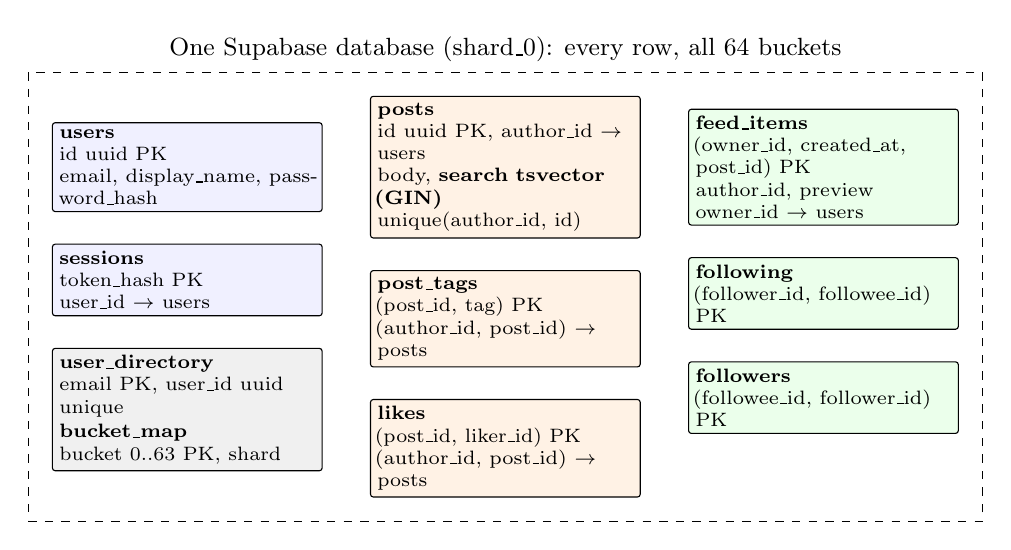
\begin{tikzpicture}[font=\scriptsize, node distance=4mm,
  tbl/.style={draw, rounded corners=1pt, fill=#1, align=left, inner sep=2.5pt, text width=3.25cm},
  tbl/.default=white]
\node[tbl=blue!6] (u) {\textbf{users}\\ id uuid PK \\ email, display\_name, password\_hash};
\node[tbl=blue!6, below=of u] (s) {\textbf{sessions}\\ token\_hash PK \\ user\_id $\to$ users};
\node[tbl=orange!10, right=6mm of u] (p) {\textbf{posts}\\ id uuid PK, author\_id $\to$ users \\ body, \textbf{search tsvector (GIN)} \\ unique(author\_id, id)};
\node[tbl=orange!10, below=of p] (t) {\textbf{post\_tags}\\ (post\_id, tag) PK \\ (author\_id, post\_id) $\to$ posts};
\node[tbl=orange!10, below=of t] (l) {\textbf{likes}\\ (post\_id, liker\_id) PK \\ (author\_id, post\_id) $\to$ posts};
\node[tbl=green!8, right=6mm of p] (fi) {\textbf{feed\_items}\\ (owner\_id, created\_at, post\_id) PK \\ author\_id, preview \\ owner\_id $\to$ users};
\node[tbl=green!8, below=of fi] (fw) {\textbf{following}\\ (follower\_id, followee\_id) PK};
\node[tbl=green!8, below=of fw] (fr) {\textbf{followers}\\ (followee\_id, follower\_id) PK};
\node[tbl=gray!12, below=of s] (d) {\textbf{user\_directory}\\ email PK, user\_id uuid unique \\[1pt] \textbf{bucket\_map}\\ bucket 0..63 PK, shard};
\node[draw, dashed, fit=(u)(s)(p)(t)(l)(fi)(fw)(fr)(d), inner sep=3mm, label={[font=\small]above:One Supabase database (shard\_0): every row, all 64 buckets}] {};
\end{tikzpicture}
\caption{Before: the extended single-database model (schema \texttt{m6}). Blue = owner tables;
orange = rows owned by the author; green = copies and follow edges; grey = directory.}
\label{fig:before}
\end{figure}

\subsection{After: the same tables, hash-partitioned over two databases}
\begin{figure}[H]\centering
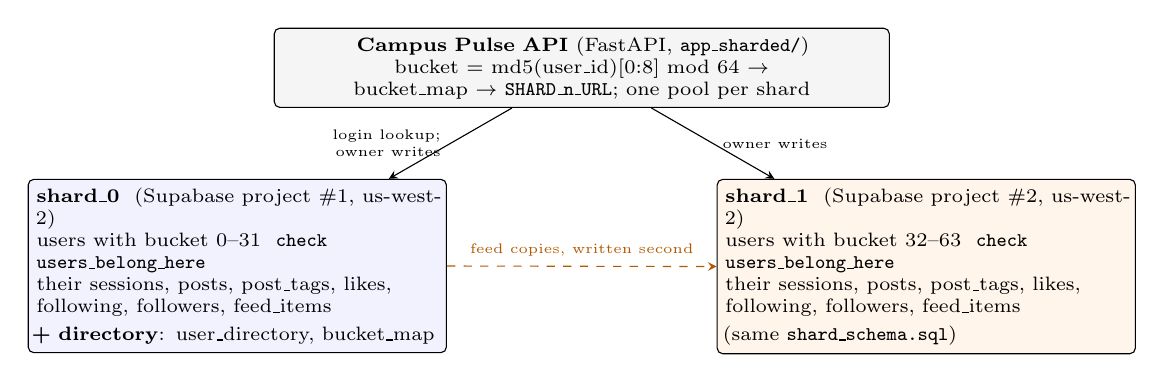
\begin{tikzpicture}[font=\scriptsize, >=stealth,
  box/.style={draw, rounded corners=2pt, align=center, inner sep=3pt},
  db/.style={draw, rounded corners=2pt, align=left, inner sep=3pt, text width=5.1cm, fill=#1},
  db/.default=white]
\node[box, fill=gray!8, text width=7.6cm] (app) {\textbf{Campus Pulse API} (FastAPI, \texttt{app\_sharded/})\\
  bucket = md5(user\_id)[0:8] mod 64 $\to$ bucket\_map $\to$ \texttt{SHARD\_n\_URL}; one pool per shard};
\node[db=blue!5, below left=9mm and -2.2cm of app] (s0) {\textbf{shard\_0} \ (Supabase project \#1, us-west-2)\\
  users with bucket 0--31 \ \texttt{check users\_belong\_here}\\
  their sessions, posts, post\_tags, likes,\\ following, followers, feed\_items\\[2pt]
  \textbf{+ directory}: user\_directory, bucket\_map};
\node[db=orange!8, below right=9mm and -2.2cm of app] (s1) {\textbf{shard\_1} \ (Supabase project \#2, us-west-2)\\
  users with bucket 32--63 \ \texttt{check users\_belong\_here}\\
  their sessions, posts, post\_tags, likes,\\ following, followers, feed\_items\\[2pt]
  (same \texttt{shard\_schema.sql})};
\draw[->] (app) -- node[left, font=\tiny, align=right]{login lookup;\\ owner writes} (s0);
\draw[->] (app) -- node[right, font=\tiny, align=left]{owner writes} (s1);
\draw[->, dashed, orange!70!black] (s0.east) -- node[above, font=\tiny]{feed copies, written second} (s1.west);
\end{tikzpicture}
\caption{After: two Supabase projects in the same region. Each database owns half of the users and
every row those users own. A post commits on the author's shard; copies for followers on the other shard
are written second (and retried) by \texttt{m6.fanout()}.}
\label{fig:after}
\end{figure}

\noindent Differences between the before and after models, table by table:
\begin{itemize}[nosep,leftmargin=1.2em]
\item \textbf{Same shape, different rows:} all eight data tables exist on both shards; a row's home is
      computed from its owner's id. Integer serial ids (M1) became UUIDs so no shared counter is needed.
\item \textbf{New routing columns:} \texttt{likes.author\_id} and \texttt{post\_tags.author\_id} let child rows
      follow the post's owner; composite foreign keys \texttt{(author\_id, post\_id)} $\to$ \texttt{posts(author\_id, id)}
      guarantee a child can only attach to a post on the same shard.
\item \textbf{Cross-owner relations became two rows:} M1's \texttt{friendships} became \texttt{following}
      (follower's shard) + \texttt{followers} (followee's shard); \texttt{likes.liker\_id} has no foreign key because
      the liker may live elsewhere.
\item \textbf{New central-but-small tables} on shard\_0 only: \texttt{user\_directory} (email uniqueness and
      login lookup) and \texttt{bucket\_map}. They are touched only at registration and login.
\item \textbf{Fail loudly:} each shard's \texttt{users} table rejects ids from the other shard's buckets.
\end{itemize}

\section{Implementation: the ten steps on Supabase}\label{sec:steps}

We followed ``How to shard in Azure + Supabase'' step by step and adapted the handout
\texttt{sharding\_setup.sql} (Part A and the social-media appendix). Our app runs on Render, not Azure
App Service, and for the load tests it ran on a lab server, so ``Azure app settings'' became environment variables
(Step~7). All objects live in a dedicated schema \texttt{m6} so the M1/M2 tables in \texttt{public} keep serving
the hosted M1 application.

\begin{center}\small
\begin{tabularx}{\linewidth}{@{}r>{\raggedright}p{4.1cm}>{\raggedright\arraybackslash}X@{}}
\toprule
Step & Lecture instruction & What we did (file) \\
\midrule
1 & Confirm writes are the bottleneck & \texttt{pg\_stat\_statements} (already enabled in schema \texttt{extensions}),
  reset before each series; the handout query plus a top-statement query (\texttt{m6/sql/step1\_measure.sql});
  results in Section~\ref{sec:bottleneck}. \\
2 & Write down where every table goes & Worksheet Step~5 (Section~\ref{sec:worksheet}); 64 buckets. \\
3 & One Supabase project per shard, same region & \texttt{campus-pulse-csce553} (shard\_0) and
  \texttt{campus-pulse-shard-1} (shard\_1), both \textbf{West US (Oregon), us-west-2}, Nano compute, free plan. \\
4 & Same schema file on every shard & \texttt{m6/sql/shard\_schema.sql} (bucket function, 8 tables, \texttt{publish\_post()}, \texttt{fanout()}). \\
5 & Check that rejects other shards' users & \texttt{m6/sql/shard\_check.sql}: \texttt{users\_belong\_here} with 0--31 / 32--63
  (0--63 in the one-database baseline). \\
6 & Directory and bucket map on shard\_0 & \texttt{m6/sql/directory.sql}: \texttt{user\_directory}, \texttt{bucket\_map} (32/32). \\
7 & Connection strings in settings, not code & \texttt{SHARD\_0\_URL}, \texttt{SHARD\_1\_URL} in \texttt{.env} (git-ignored);
  the app maps the \texttt{bucket\_map} name \texttt{shard\_1} to \texttt{SHARD\_1\_URL}. Session-pooler strings (IPv4);
  the app uses the same pooler's transaction port 6543. \\
8 & Load shared products on every shard & Not applicable: Campus Pulse has no shared catalogue. The only
  thing that must be identical everywhere is \texttt{shard\_bucket()}, which we verify (Python = SQL for 2{,}000 ids on every shard). \\
9 & Writes: route by owner & register (directory row, then user row on its shard, retried with the same id);
  publish (\texttt{publish\_post()} on the author's shard, then \texttt{fanout()} copies on other shards);
  like (row on the post author's shard); follow (two idempotent writes). \texttt{app\_sharded/main.py} \\
10 & Reads: find the shard, then plain SQL & login looks up \texttt{user\_directory}$\bowtie$\texttt{bucket\_map} once; the session token is
  \texttt{shard\_n.<random>}, so every per-user page (home feed, following, my posts) is a one-shard query. \\
\bottomrule
\end{tabularx}
\end{center}

\subsection*{Adapted SQL (excerpts)}
The bucket rule and the shard check are unchanged from the handout except for the schema name:
\begin{lstlisting}[language=SQL]
create or replace function m6.shard_bucket(u uuid) returns int language sql immutable as $$
  select (('x' || substr(md5(u::text), 1, 8))::bit(32)::bigint % 64)::int $$;
alter table m6.users add constraint users_belong_here
  check (m6.shard_bucket(id) between 0 and 31);          -- 32..63 on shard_1
\end{lstlisting}
Publishing is the social-media equivalent of the handout's \texttt{checkout()}: one stored procedure, one local
transaction on the owner's shard. It returns the followers that live on other shards so the app can write their
copies second:
\begin{lstlisting}[language=SQL]
create or replace function m6.publish_post(p_post uuid, p_author uuid, p_body text, p_tags text[],
    out post_created_at timestamptz, out remote_followers uuid[]) language plpgsql as $$
begin
  post_created_at := clock_timestamp();
  insert into m6.posts (id, author_id, body, created_at, updated_at)
  values (p_post, p_author, p_body, post_created_at, post_created_at);
  insert into m6.post_tags (author_id, post_id, tag)
  select p_author, p_post, t from unnest(p_tags) t on conflict do nothing;
  insert into m6.feed_items (owner_id, created_at, post_id, author_id, preview)      -- local copies
  select x.owner, post_created_at, p_post, p_author, left(p_body, 80)
  from (select p_author as owner union
        select f.follower_id from m6.followers f where f.followee_id = p_author) x
  where exists (select 1 from m6.users u where u.id = x.owner);
  select coalesce(array_agg(f.follower_id), '{}') into remote_followers        -- for fanout()
  from m6.followers f where f.followee_id = p_author
   and not exists (select 1 from m6.users u where u.id = f.follower_id);
end $$;
\end{lstlisting}
Registration follows Step~9 exactly (A on the directory, B on the returned shard), and a like is the appendix
statement with the routing column added:
\begin{lstlisting}[language=SQL]
insert into m6.user_directory (email) values (lower(:email)) returning user_id;   -- A, shard_0
insert into m6.users (id, email, display_name, password_hash) values (...)        -- B, user's shard
  on conflict (id) do nothing;                                                    -- retry-safe
insert into m6.likes (author_id, post_id, liker_id) values (...) on conflict do nothing;
\end{lstlisting}

\section{Load-test method}\label{sec:method}

\paragraph{System under test.} The load driver and the API run on one lab server (32 cores, 188~GB RAM). The API
is \texttt{app\_sharded} under uvicorn with 6 worker processes. Each worker holds a \texttt{psycopg} pool of up to
32 connections per shard to the Supabase transaction pooler (port 6543), so a project sees at most 192 client
connections, below the pooler's limit of 200; Supabase maps them onto 15 server connections per Nano project.
Databases: Supabase free plan, Nano compute (2 vCPU), PostgreSQL 17, both in us-west-2 (Render's default Oregon region
is the same). The median \texttt{SELECT 1} round trip from the server was 73~ms to shard\_0 and 75~ms to shard\_1. We
sized the API so that it is not the first limit and checked this (Section~\ref{sec:apifirst}).

\paragraph{Two series, one variable.} Series \textbf{S1 (before)}: \texttt{ACTIVE\_SHARDS=1}, all 64 buckets on
shard\_0. Series \textbf{S2 (after)}: \texttt{ACTIVE\_SHARDS=2}, buckets 0--31 on shard\_0 and 32--63 on shard\_1.
Both series use the same code and the same seed: each rebuilds schema \texttt{m6} and loads the same 400 users
(fixed random seed 553), the same 16{,}000 follow edges (40 per user) and one session token per user, then runs
\texttt{m6/run\_series.py}. SHA-256 hashes of the code are stored with the results.

\paragraph{Driver.} \texttt{m6/load\_m6.py} keeps the M2 driver's closed-loop design and statistics: warm-up
discarded, fixed measurement window, per-request CSV, p50/p95/p99/max and error rate. Sharding needed two changes.
Every client is a \emph{different} user, because one shared token, as in M2, would put all writes on one owner and
therefore on one shard. Concurrency goes up to 256.

\paragraph{Stages.} The publish staircase uses $c=1,4,8,16,32,64,128,256$ clients. Each stage has 5~s of warm-up and
30~s of measurement; then all posts and feed rows are truncated and the system recovers for 15~s, so every stage
starts with the same table sizes. The stop rule is the same as in M2: error rate $>$10\% or p99 $>$5~s (never
triggered). After the staircase come a repeat of $c=128$, and like-only, home-feed-read and a 70/20/10 read/like/post
mix at $c=128$, run against 2{,}000 pre-loaded like targets and pre-filled feeds. We later added intermediate publish
stages to locate each peak, with the same protocol (\texttt{m6/run\_extra.py}): $c=48,96$ for S1, and $c=96,160,192$
plus a repeat of $c=256$ for S2.
The 30~s window (M2 used 60~s) keeps one-database stages under the free plan's 500~MB limit: each post leaves
$\approx$13~KB of rows and index entries, and the single database reaches $\approx$575 posts/s.

\paragraph{Database-side evidence.} During every measured window, on every shard, the driver records:
\begin{itemize}[nosep,leftmargin=1.2em]
\item 1~Hz samples of \texttt{pg\_stat\_activity}: active client backends and their wait events;
\item before/after deltas of three statistics views: commits and rows inserted (\texttt{pg\_stat\_database}),
      WAL bytes (\texttt{pg\_stat\_wal}), and the calls and execution time of every \texttt{m6} statement
      (\texttt{pg\_stat\_statements}).
\end{itemize}
Host CPU, iowait and disk writes of each database VM come from Supabase's Prometheus endpoint
(\texttt{/customer/v1/\allowbreak privileged/\allowbreak metrics}), which refreshes about every 60~s and is logged continuously by
\texttt{m6/metrics\_logger.py}. API CPU is the sum over the uvicorn master and its workers (psutil, sampled every 2~s).

\paragraph{Functional check.} \texttt{m6/smoke\_test.py} exercises Steps~9--10 over HTTP on the two-shard layout:
registration lands users on both shards, a duplicate email is rejected, login returns the user's shard, a cross-shard follow writes
both rows, a post's feed copy is written on the other shard, likes go to the author's shard, only the author can edit,
forged tokens are rejected, and a wrong-shard insert is rejected. All 16 checks pass (\texttt{results/smoke-S2.json}).

\paragraph{Other controls.} M5's pg\_cron job (refresh \texttt{search.post\_search} every 5 minutes) was paused
during each series and re-enabled afterwards. The M1/M2 tables in \texttt{public} and the hosted Render service were
not modified.

\section{Results}\label{sec:results}

\subsection{First, make sure the database is what saturates}\label{sec:apifirst}
Our first two attempts did not measure the database. With 8 API workers $\times$ 8 pooled connections the publish
curve flattened at $\approx$300 posts/s, but the database had only 3.5--5 busy backends and a home-feed
\emph{read}, which barely touches the database, was capped at the same $\approx$380 requests/s: the API's
connection pool was the bottleneck (each request holds a connection for a 75~ms round trip). Raising the pool to
16$\times$12 moved the plateau to $\approx$460 posts/s with the same symptom. With the final setting (6 workers
$\times$ 32 connections per shard; at most 192 client connections per project, below the Supabase pooler's 200)
a feed read reaches 1{,}571 requests/s and a like 1{,}330 requests/s through the same API with the database almost idle,
while publish saturates at $\approx$574 posts/s. The request path can therefore carry at least 2.7$\times$ the
publish throughput we report, so the publish plateau below is a database limit. The superseded runs are kept in
\texttt{m6/results-run1-apipool/} and \texttt{m6/results-run2-api16x12/}.

\subsection{Before sharding: writes are the bottleneck}\label{sec:bottleneck}

\begin{figure}[H]\centering
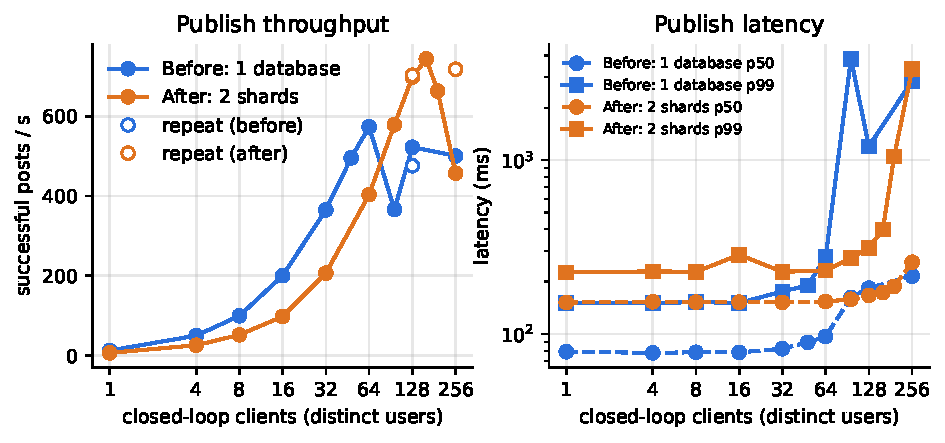
\includegraphics[width=\linewidth]{figures/post_throughput_latency.pdf}
\caption{Publish staircase, one database (blue) vs.\ two shards (orange). Hollow points are repeated stages.
Each point is a 30~s closed-loop stage with distinct users; zero errors in every stage.}
\label{fig:tput}
\end{figure}

\paragraph{Throughput and latency.} With one database, publish throughput grows linearly up to 32 clients
(365 posts/s, p99 176~ms), peaks at \textbf{574 posts/s at 64 clients} (25{,}600 rows inserted/s, 10.8~MB/s of WAL),
and then \emph{falls} as more writers are added: 522 posts/s at 128 clients and 501 at 256, while p99 rises from
276~ms to 1.2~s and 2.9~s. The 96-client stage was unstable (366 posts/s, p99 3.8~s). The repeated 128-client stage
gave 476 posts/s, 9\% below the first run; the shared Nano instance is noisy once it is overloaded. More clients past
the knee only add queueing; Little's law holds in every stage (Table~\ref{tab:little}).

\paragraph{Where the time goes inside the database.} The 1~Hz \texttt{pg\_stat\_activity} samples
(Figure~\ref{fig:waits}) show the number of busy backends rising from 1.5 (16 clients) to 14--15.6 (64 clients and
above), which is the Supabase pooler's 15 server connections for a Nano project. On a 2-vCPU machine, 7--10 of them are
runnable on CPU, and 3--4 wait on \texttt{LWLock:WALWrite} / \texttt{IO:WalSync}, i.e.\ for their commit record to
reach disk, plus 1--3 on buffer-content and relation-extension locks. The same statement got slower as load rose:
the mean execution time of \texttt{publish\_post()} went from 3.4~ms (16 clients) to 7.0, 11.6, 16.8 and 22--24~ms
(32, 48, 64, $\ge$128 clients). The work per post did not change (46 rows, one commit), so this 7$\times$ slowdown is contention.

\begin{figure}[H]\centering
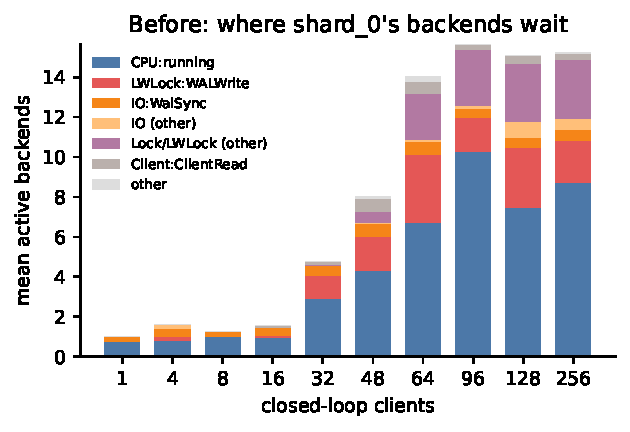
\includegraphics[width=0.56\linewidth]{figures/waits_before.pdf}\hfill
\begin{minipage}[b]{0.42\linewidth}\small
\captionof{figure}{One database: mean number of active backends by wait event (1~Hz samples). Blue = on CPU;
red/orange = waiting for the WAL to be written and flushed (commit).}\label{fig:waits}
\vspace{6mm}
\end{minipage}
\end{figure}

\paragraph{The host.} Supabase's metrics endpoint refreshes about every 60~s, so we logged it continuously and plot
it against the stage windows (Figure~\ref{fig:hostS1}). During the saturated publish stages (64--256 clients) the database VM spent
34--61\% of its CPU in user+system time and another 18--44\% in \textbf{iowait}; busy+iowait stayed at 73--79\%,
leaving about 20\% idle, and it wrote 16--21~MB/s to disk. The two cores are either computing inserts and index updates or waiting for the disk.

\begin{figure}[H]\centering
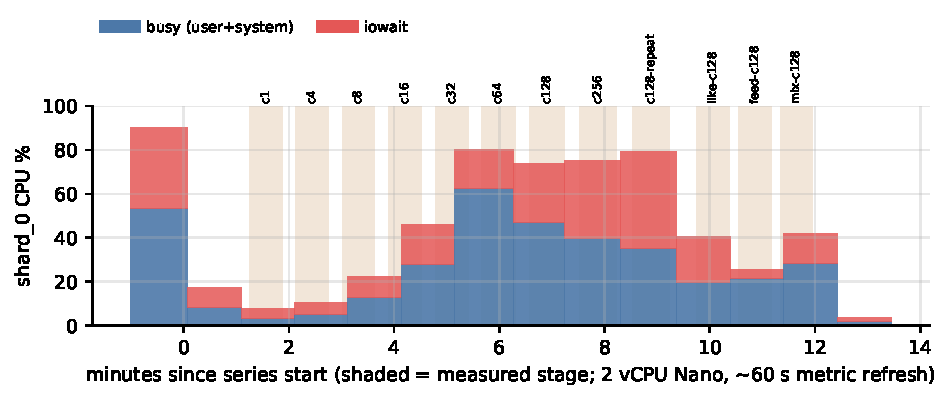
\includegraphics[width=\linewidth]{figures/host_cpu_S1.pdf}
\caption{One database: shard\_0 VM CPU per metrics refresh (blue = user+system, red = iowait). Shaded bands are the measured stages.}
\label{fig:hostS1}
\end{figure}

\paragraph{Step 1 query.} The handout query (statements starting with INSERT/UPDATE/DELETE) returns no rows for
Campus Pulse, because every busy write runs inside a stored procedure called with \texttt{SELECT}. Over all
statements, \texttt{publish\_post()} accounts for 98.8\% of the execution time of the top ten statements and wrote
1.53~GB of WAL during the one-database staircase:

\begin{center}\scriptsize
\begin{tabular}{@{}llrrrr@{}}
\toprule
Shard & Statement (\texttt{pg\_stat\_statements}, after the S1 staircase) & Calls & Total ms & Mean ms & WAL MB \\
\midrule
\tabinput{tables/step1_S1.tex}
\bottomrule
\end{tabular}
\end{center}

\noindent\textbf{Conclusion for Step 1:} writes are the bottleneck. The top statement is the write path, the
database runs out of connections, CPU and commit bandwidth, more clients make throughput worse, and the cheaper fixes
from slide~25 are already in place (one stored-procedure call per post, no counter row, no unused index). The next
cheapest fix would be a bigger compute plan; the assignment asks us to shard.

\subsection{After sharding: the same staircase on two databases}

\begin{figure}[H]\centering
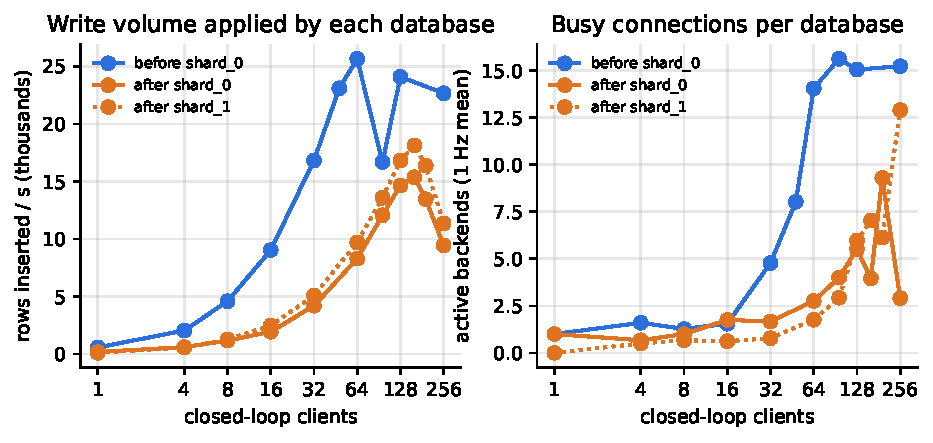
\includegraphics[width=\linewidth]{figures/db_per_shard.pdf}
\caption{Rows inserted per second and busy backends, per database. After sharding, each database applies about half
of the rows, and neither database reaches the 15-backend ceiling at the throughputs where the single database is saturated.}
\label{fig:pershard}
\end{figure}

\paragraph{Capacity.} With two shards, publish peaks at \textbf{744 posts/s at 160 clients} (p99 398~ms), and stays at
698--744 posts/s from 128 to 160 clients with p99 $\le$ 400~ms. The one-database peak was 574 posts/s with p99 276~ms. The
peak is 1.30$\times$ higher, and over the saturated region the median is 700 vs.\ 501 posts/s (1.40$\times$). At 192 and 256 clients the
two-shard system also overloads (663 and 457/718 posts/s, p99 up to 3.3~s; the two 256-client runs differ by 57\%).

\paragraph{Load per database.} Compare stages with the same throughput: one database at 64 clients (574 posts/s) and two
shards at 96 clients (579 posts/s). Each shard inserted 12.1k and 13.6k rows/s instead of 25.6k, had 4.0 and 2.9 busy
backends instead of 14.1, and ran \texttt{publish\_post()} in 3.5~ms instead of 16.8~ms. Halving the rows per database
removed most of the contention, so each shard is far below its own saturation point while carrying the same user load.

\paragraph{Latency at low load got worse.} At 1--64 clients, two shards deliver about half the throughput of one database
at the same concurrency (403 vs.\ 574 posts/s at 64 clients), and p50 rises from 78 to 153~ms. The cause is the
cross-shard copy: a post now commits on the author's shard and then writes follower copies on the other shard,
written second as the lecture requires, so one click costs two sequential 75~ms round trips. Closed-loop throughput
at fixed concurrency is $c/R$, so it halves until the databases saturate.

\begin{figure}[H]\centering
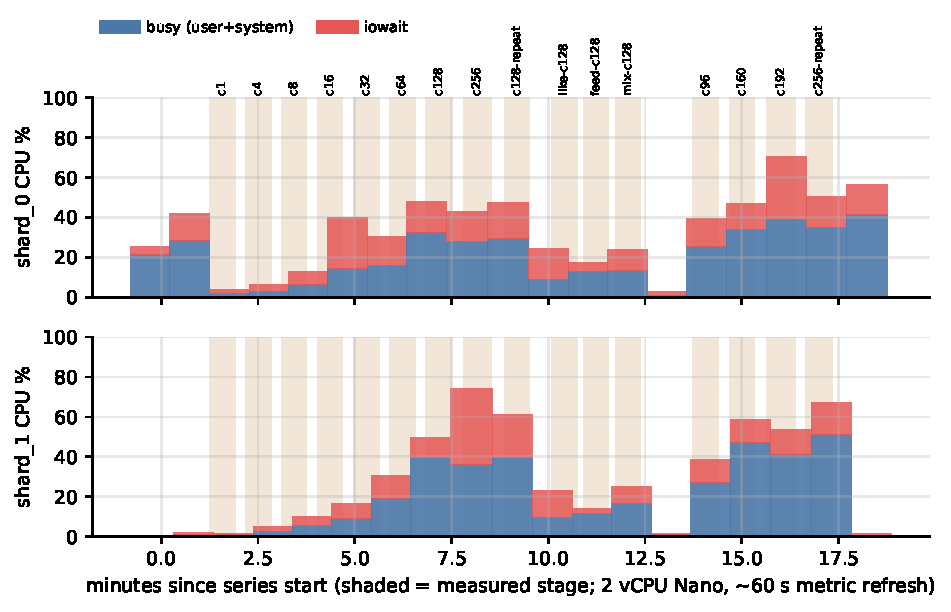
\includegraphics[width=\linewidth]{figures/host_cpu_S2.pdf}
\caption{Two shards: VM CPU of both databases. In the 128-client stages both are around 45--50\% busy+iowait; the
first 256-client stage drove shard\_1 to 74\% (iowait 38\%) while shard\_0 stayed near 43\%.}
\label{fig:hostS2}
\end{figure}

\paragraph{The busiest shard decides.} shard\_1 owns 219 of the 400 users (55\%; buckets are hashed, so the split is
close but not exact) and therefore receives 24 rows per post vs.\ 21 on shard\_0. In the first 256-client stage shard\_1's
\texttt{publish\_post()} took 22.9~ms and it had 12.9 busy backends, while shard\_0 had 2.9. Every post waits for both
shards, so the slower shard set the throughput (457 posts/s). This is lecture slide~15: capacity is the busiest
shard.

\paragraph{Other workloads (128 clients).}
\begin{center}\footnotesize
\begin{tabular}{@{}lrrrrl@{}}
\toprule
Workload & 1 DB req/s & 2 shards req/s & Change & p99 (1 DB $\to$ 2) & Note \\
\midrule
Like (1-row insert) & 1{,}330 & 1{,}609 & +21\% & 188 $\to$ 148 ms & commit waits gone; API ceiling \\
Home-feed read & 1{,}571 & 1{,}636 & +4\% & 149 $\to$ 148 ms & DB nearly idle in both \\
70/20/10 mix & 1{,}553 & 1{,}484 & $-$4\% & 150 $\to$ 160 ms & posts pay a 2nd round trip \\
\bottomrule
\end{tabular}
\end{center}
Reads did not get faster, and the lecture says they should not: sharding adds write capacity. The home feed remained a
one-shard query because its rows are copies on the reader's shard.

\subsection{Correctness checks (lecture slide 41)}
\begin{center}\small
\begin{tabular}{@{}lll@{}}
\toprule
Check & Result (two shards) & Expected \\
\midrule
Users per shard (\texttt{count(*)} on each) & shard\_0: 181, shard\_1: 219 & close, not identical \\
Users per shard via directory $\bowtie$ bucket\_map & shard\_0: 181, shard\_1: 219 & same as above \\
Rows on the wrong shard & 0 and 0 & 0 \\
\texttt{bucket\_map} & 32 / 32 buckets & 32 / 32 \\
Bad insert (bucket 37) on shard\_0 & rejected: violates \texttt{users\_belong\_here} & rejected \\
Python \texttt{shard\_bucket} vs.\ SQL, 2{,}000 ids & identical on both shards & identical \\
\bottomrule
\end{tabular}
\end{center}

\subsection{All stages}
Per-stage results; for two shards, per-database columns are given as shard\_0 / shard\_1. ``Exec'' = seconds of
statement execution per second (from \texttt{pg\_stat\_statements}); ``Busy'' = mean active backends; API CPU in \% of one core.
\begin{center}\scriptsize\setlength{\tabcolsep}{3pt}
\resizebox{\linewidth}{!}{%
\begin{tabular}{@{}lrrrrrrrrllll r@{}}
\toprule
Workload & $c$ & Requests & OK/s & p50 & p95 & p99 & max & Err & Rows/s (k) & Exec s/s & Busy & WAL MB/s & API \\
\midrule
\multicolumn{14}{@{}l}{\textbf{Before: one database (S1)}} \\
\tabinput{tables/stages_S1.tex}
\midrule
\multicolumn{14}{@{}l}{\textbf{After: two shards (S2)}} \\
\tabinput{tables/stages_S2.tex}
\bottomrule
\end{tabular}}
\end{center}

\begin{table}[H]\centering\small
\caption{Little's law check: in-flight requests $L = X\cdot R$ match the closed-loop client count $c$.}\label{tab:little}
\begin{tabular}{@{}rlrrrr@{}}
\toprule
Shards & Workload & $c$ & $X$ (req/s) & $R$ mean (ms) & $L = X R$ \\
\midrule
\tabinput{tables/little.tex}
\bottomrule
\end{tabular}
\end{table}

\section{Discussion}\label{sec:discussion}

\paragraph{Why not 2$\times$? Sharding split the rows, not the commits.}
Per post, the one database applied 46 rows in 1.02 commits. After sharding each database applied 21 or 24 rows
per post, about half, but still 1.03 commits per post: the author's shard commits \texttt{publish\_post()},
and the other shard commits \texttt{fanout()} for the followers who live there. With 40 random followers per
user, almost every post has followers on both shards. Commit-related waits (WALWrite, WalSync) were a large share
of the single database's saturation (Figure~\ref{fig:waits}), and the commit rate each Nano disk must sustain went from
587/s (one database at its peak) to 765/s per shard (two shards at their peak). Sharding therefore removed most of the
CPU and lock contention from inserting and indexing rows. It did not remove the per-commit cost. The
measured gain is 1.30--1.40$\times$, not the ideal 2$\times$ of an app whose writes stay with one owner (lecture
slide~9, e-commerce).

\paragraph{The cost of copy-at-write across shards.} The same design decision has a latency cost: one publish is
two sequential round trips (Section~\ref{sec:results}), so at low and medium load users see a p50 of about 155~ms instead of 78~ms.
The lecture accepts this ordering because the real record has to exist before its copies. Two fixes follow from the
lecture's own principles:
\begin{enumerate}[nosep,leftmargin=1.4em]
\item \emph{Combine many small writes into fewer} (slide~25): queue the follower copies and apply them per shard
      in batches, e.g.\ one \texttt{fanout()} transaction per shard every 50~ms carrying many posts. The post returns
      after one round trip, and the second shard's commit rate drops from one per post to one per batch.
\item \emph{Collect at read time} for authors with many followers (slide~50): no copies at all, so the publish is a
      one-shard, one-commit transaction, and the feed read asks both shards and merges.
\end{enumerate}
We did not implement these. They change the semantics (feeds become eventually consistent within the batch interval),
and the assignment asks for the lecture's ten steps.

\paragraph{Hot shard and hot owner.} With 400 users, hashing gave a 45/55 split, and the busier shard limited the
overloaded 256-client stage. More users would even this out; the lecture's 2{,}000-user test gave 1{,}008:992. One
very busy owner, the worksheet's Step~3 celebrity, cannot be split by hashing: all of its likes land on one shard.
Because likes are inserted as rows and never update a counter, they do not queue on a single row lock.

\paragraph{Revised capacity statement.} With two Nano shards, Campus Pulse sustained about 700 posts/s
($\approx$31{,}000--33{,}000 rows/s across both databases) with p99 $\le$ 400~ms, against 574 posts/s with p99 276~ms on one Nano database.
The M2 1M-user model needs about 17 posts/s (10\% of 167 write RPS). Both configurations cover that, so for
Campus Pulse at class scale sharding would be premature (``shard last'', slide~25). The numbers show what sharding
buys once a single database is saturated: about 1.3--1.4$\times$ for this fan-out-heavy write. Writes that touch one
owner (likes, sessions) should scale closer to 2$\times$, but our like test reached the API's $\approx$1{,}600~req/s ceiling
before either shard saturated (+21\%), so we did not measure their limit.

\paragraph{Confounds and limits.}
\begin{itemize}[nosep,leftmargin=1.2em]
\item \textbf{Shared free-tier hardware.} Nano projects run on shared hosts. Overloaded stages varied by up to 57\%
      between repeats (256 clients, two shards); unsaturated stages repeated within 1\% (128 clients, two shards:
      698 vs.\ 703 posts/s). We report repeats instead of averaging them.
\item \textbf{30~s measurement windows} (M2 used 60~s) because a one-database stage writes $\approx$13~KB per post and
      must stay below the 500~MB free-plan limit. Every stage starts from truncated tables.
\item \textbf{Host metrics have 60~s resolution and are not aligned with stages}, so we show them as a timeline and use
      the in-database 1~Hz samples for per-stage claims.
\item \textbf{Two different Postgres patch versions} (17.6 on shard\_0, 17.11 on shard\_1); same region, same compute size;
      round-trip times 73 and 75~ms.
\item \textbf{Load generator and API on one lab server}, 75~ms from Supabase. The API ceiling (about 1{,}600 req/s for
      requests that barely touch the database) is above every publish result we report. Hosted Render was not used
      for M6 because its single free instance tops out near 15 requests/s (M2).
\item \textbf{Closed-loop, uniform workload}: 40 followers per user and one fixed post body with three hashtags. Real
      follower counts are skewed, which would make the hot-owner effects larger.
\end{itemize}

\paragraph{Housekeeping.} The M4/M4b experiment schemas (about 415~MB) were exported to compressed CSV and dropped
from shard\_0 to make room; the M1/M2 \texttt{public} tables, the M5 \texttt{search} schema and the hosted app were
not modified, and M5's cron refresh was re-enabled after each series.

\section{Reproduction}\label{sec:repro}
\begin{lstlisting}[language=bash]
python -m venv .venv && source .venv/bin/activate
pip install -r requirements-dev.txt -r m2/requirements.txt
# .env (git-ignored): SHARD_0_URL=postgresql://postgres.<ref0>:<pw>@aws-0-us-west-2.pooler.supabase.com:5432/postgres
#                     SHARD_1_URL=postgresql://postgres.<ref1>:<pw>@aws-0-us-west-2.pooler.supabase.com:5432/postgres
python m6/run_series.py --shards 1     # before: one database (rebuilds schema m6, seeds, runs all stages)
python m6/run_series.py --shards 2     # after: two shards
python m6/run_extra.py --shards 2 --steps 96,160,192 --repeat 256    # intermediate stages
python m6/run_extra.py --shards 1 --steps 48,96 --reseed
m6/serve.sh 2 2 8602 & python m6/smoke_test.py   # functional check of Steps 9-10 (2-shard layout)
python m6/report/build.py              # figures + tables from m6/results/*.json
cd m6/report && latexmk -pdf main.tex
# manual steps: python m6/shardctl.py setup|seed|check --shards 2 ; m6/serve.sh 2 6 8600
\end{lstlisting}
Raw evidence in \texttt{m6/results/}: per-request CSVs (\texttt{*.requests.csv}), 1~Hz wait-event samples
(\texttt{*.dbwait.csv}), API CPU (\texttt{*.apicpu.csv}), per-stage JSON with database deltas, \texttt{summary.csv},
\texttt{timeline.jsonl} (UTC), the shard checks (\texttt{S1-check.json}, \texttt{S2-check.json}), the Step~1 statement
statistics (\texttt{step1-S1.json}, \texttt{step1-S2.json}), the functional check (\texttt{smoke-S2.json}), the
host-metrics log (\texttt{dbhost-timeline.jsonl}) and SHA-256 fingerprints of the code that produced them.
Session tokens and connection strings stay in the git-ignored \texttt{m6/.private/} and \texttt{.env}.


\end{document}
